\subsubsection{Adaptive Thresholding}\label{sec: Adaptive Thresholding}
The TIFF images often vary in intensity, distribution and scaling of the height profile of the DNA samples. This presents a couple of problems for the thresholding algorithms, such as pollution of some image regions which distort the threshold. As discussed above, these issues lead to a false classification of the DNA strands or even to a complete loss of image information.
Two sorts of noise persist after the initial pipelining steps  
Opencv Denoising, LowPassFilter and Median Filter (see Sections \ref{sec:Denoising}, \ref{sec:Filtering}).
\begin{figure}[!htb]
	\begin{subfigure}{0.5\textwidth}
		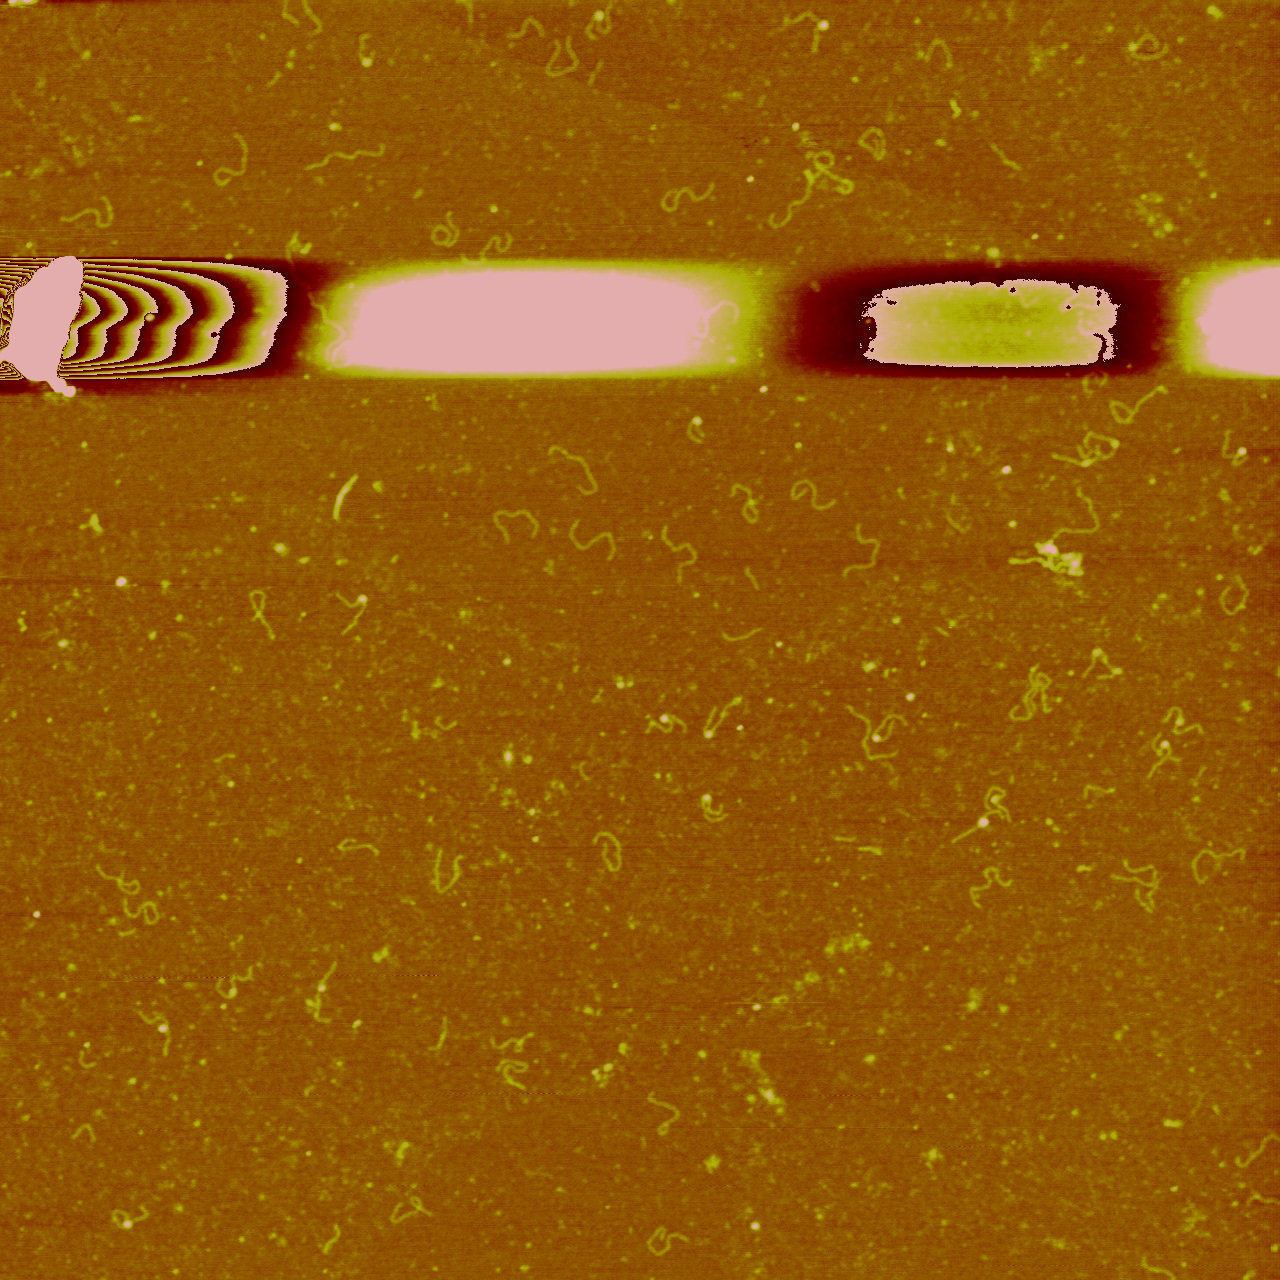
\includegraphics[width=\linewidth]{noise1.png}
		\caption{}
		\label{fig: Noise1}
	\end{subfigure}%
	\hspace{\fill}
	\begin{subfigure}{0.5\textwidth}
		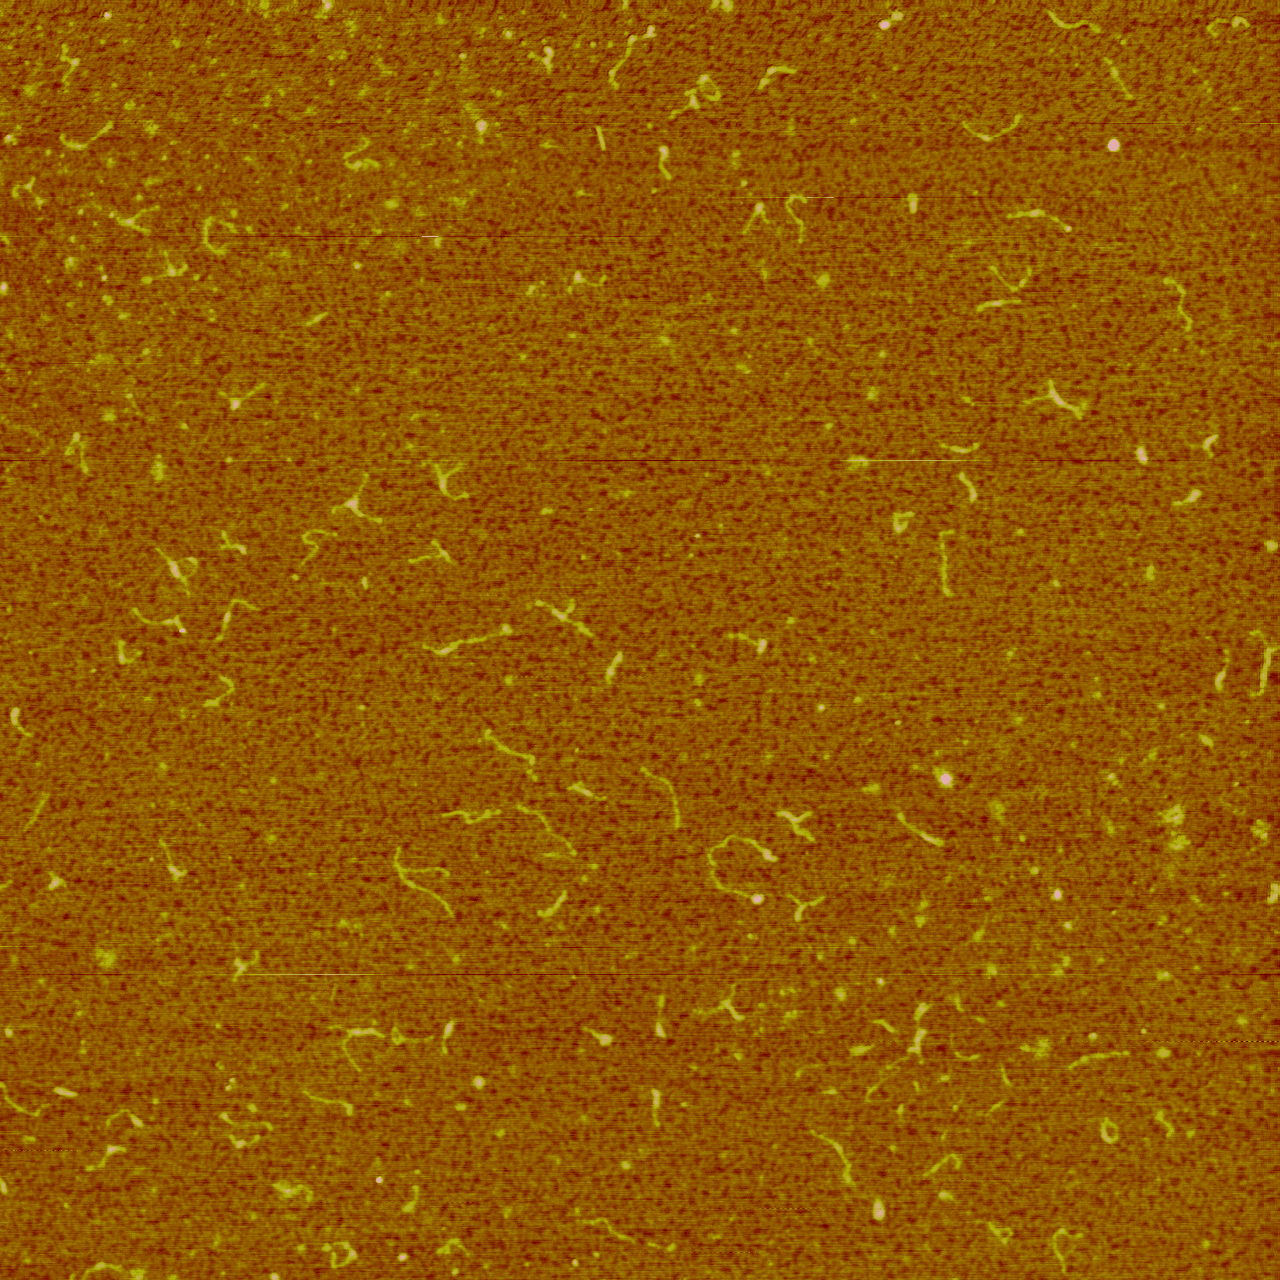
\includegraphics[width=\linewidth]{noise2.png}
		\caption{}
		\label{fig: Noise2}
	\end{subfigure}%
	\caption{(a)Noise Example 1 (b)Noise Example 2}\label{fig:Noise1Noise2}
\end{figure}
\\
The first type of noise as seen in Figure \ref{fig: Noise1} are large distorted regions in the upper value range at an approximate height of 190. If not handled these regions lift the threshold to a level where DNA-strands are missed entirely. 
The second sort of noise seen in Figure \ref{fig: Noise2} consists of small imperfections scattered over the whole image.
Unfortunately the height profile of these imperfections is very similar to the one of the DNA-strands and it is therefore very hard to automatically distinguish between them.
The overwhelming majority of disturbance on the images observed is part of the first type.
The aim of this part of the pipeline is to pre-process the data by three additional steps which treat the outliers in the upper value range and if possible improve detection and removal of scattered noise.

In order to tackle these issues the following three step method is proposed:
\begin{enumerate}
	\item Homogenize the background to provide a consistent and distinguishable layer on which the DNA-strands can be recognized easily.
	\item Identify and remove polluted image regions and outliers in the upper intensity values.
	\item Limit the threshold to an appropriate range.
\end{enumerate}
\subsubsection{Level Background}\label{sec: Level Background}

Figure \ref{fig:HistThresh} shows a histogram of the height values of a representative original image from the dataset.
In the observed dataset DNA-strands can only be found in an intensity range from about 110 to 160, while nuclei can be found between 160 and 200.


\begin{figure}[!htb]
	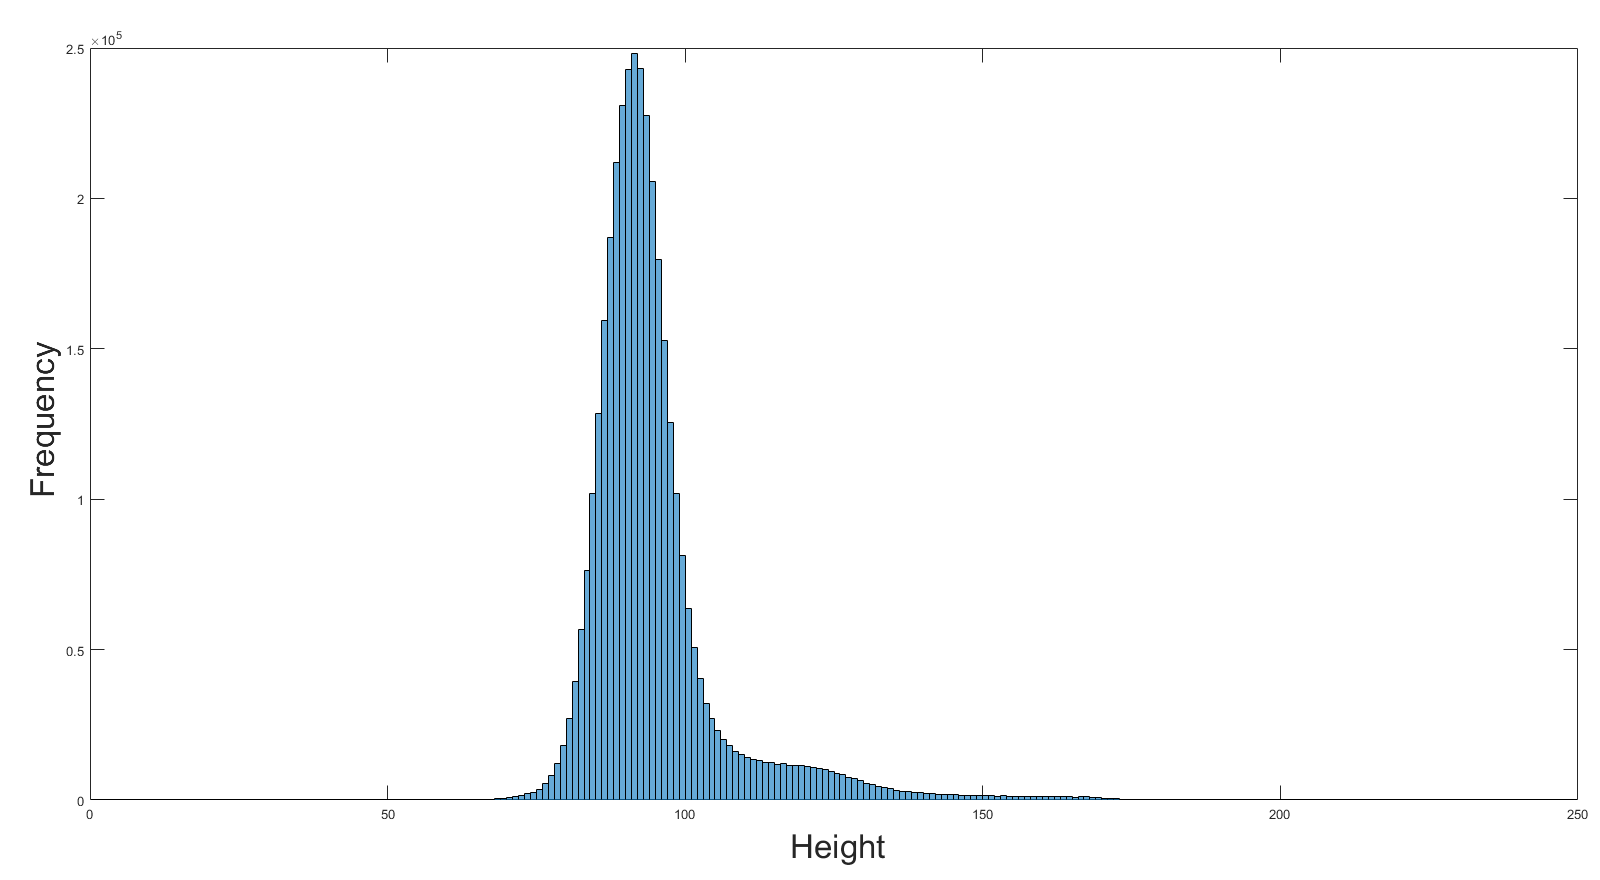
\includegraphics[width=1\linewidth]{histogramOriginal.png}
	\caption{Histogram of TIFF image}
	\label{fig:HistThresh}
\end{figure}
The accumulation point at a value of 95 is distinctive for background noise. 
Therefore, smaller values are set to this boundary.
This approach creates a more consistent background for all images and limits the variation due to noise.
It is important to mention that this method can only be used after the lowPassFilter which smooths the height distribution and thereby guarantees that only noise is removed. If applied to the raw unfiltered image this method will also remove outliers within the DNA-strands which results in perforated DNA objects.
The resulting image shown in Figure \ref{fig:background} yields a more consistent threshold and with that a higher error resistance.


\begin{figure}[!htbp]
	\begin{subfigure}{0.5\textwidth}
		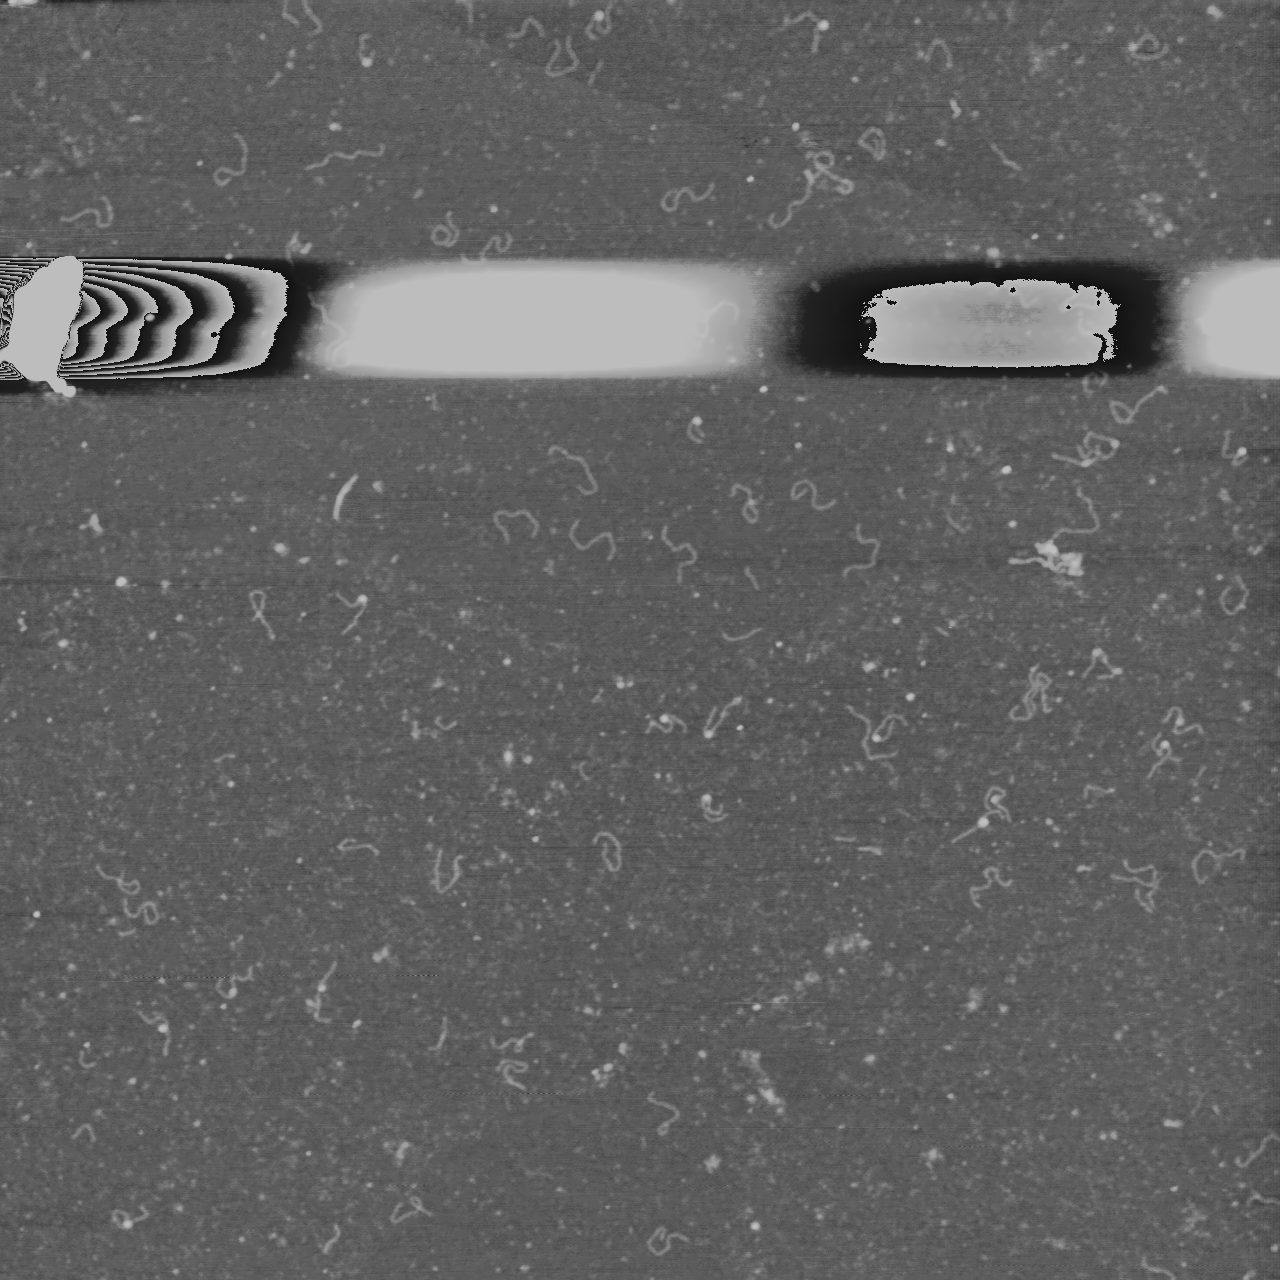
\includegraphics[width=\linewidth]{noise21.png}
		\caption{}
		\label{fig:rawImage}
	\end{subfigure}%
	\hspace{\fill}
	\begin{subfigure}{0.5\textwidth}
		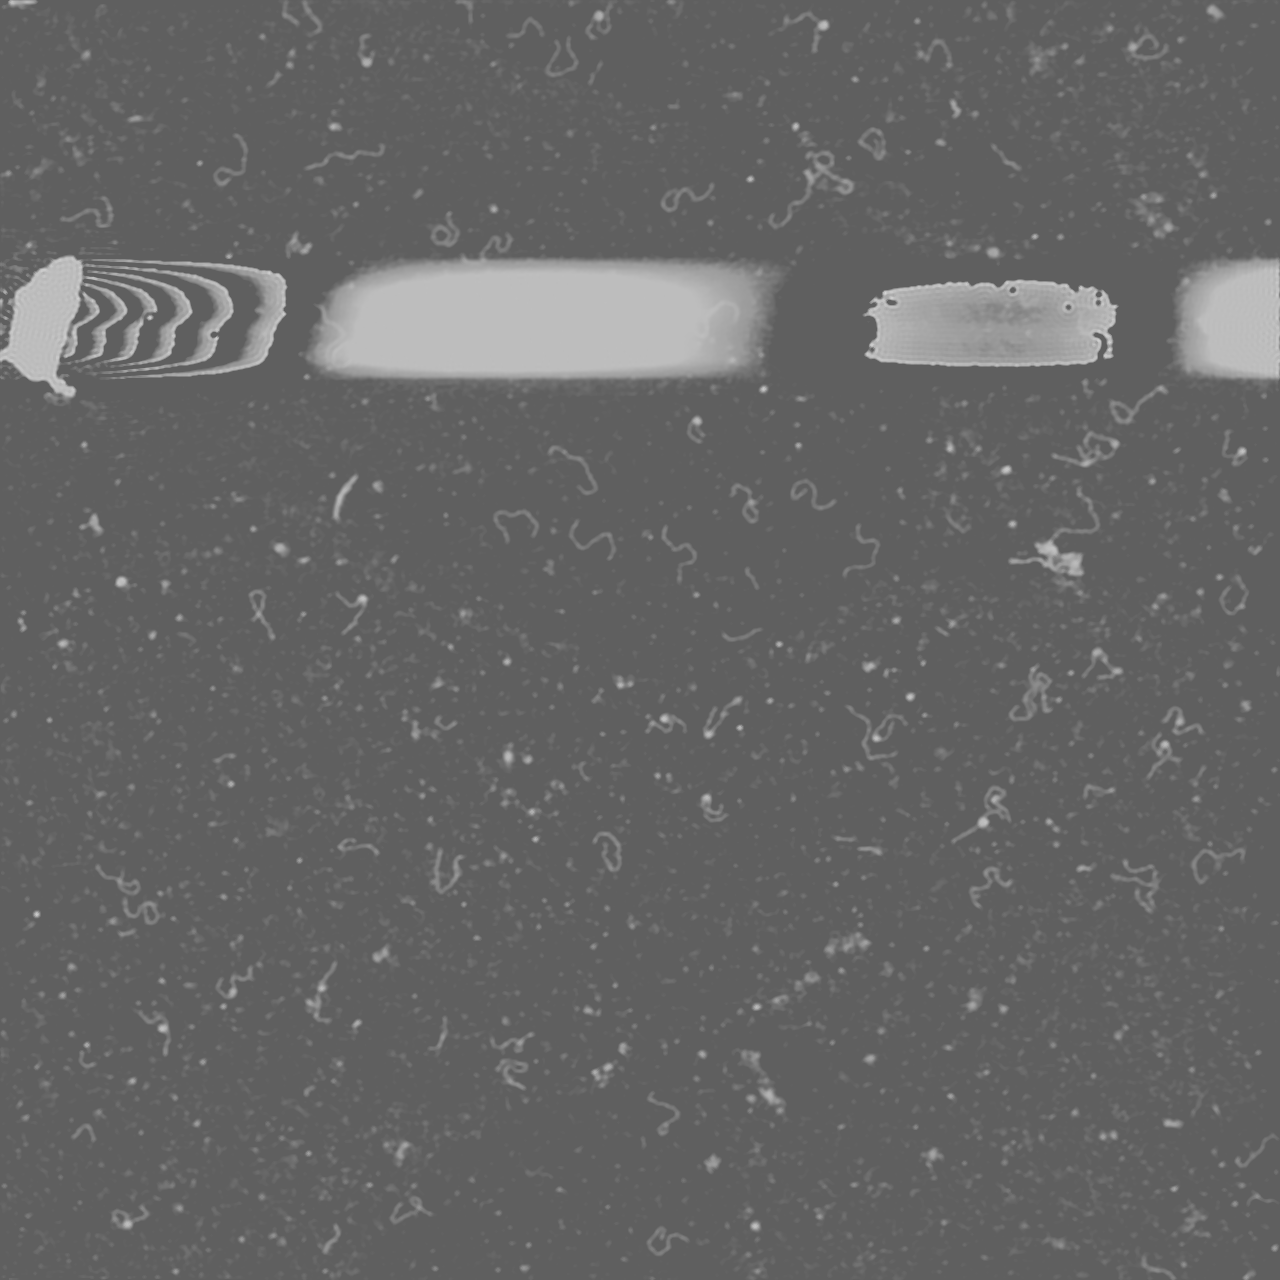
\includegraphics[width=\linewidth]{step21.png}
		\caption{}
		\label{fig:step1}
	\end{subfigure}%
	\caption{(a)Before leveling (b)After leveling }\label{fig:background}
\end{figure}
\subsubsection{Identify and remove outliers} \label{sec: Outlier Removal}
At first a global threshold algorithm like the Otsu method (see section \ref{sec:Thresholding}) is used to create a binary image.
All objects that could be a DNA object are removed based on size. Now only noise and other non-DNA objects are left.

\begin{figure}[!htb]
	\begin{subfigure}{0.5\textwidth}
		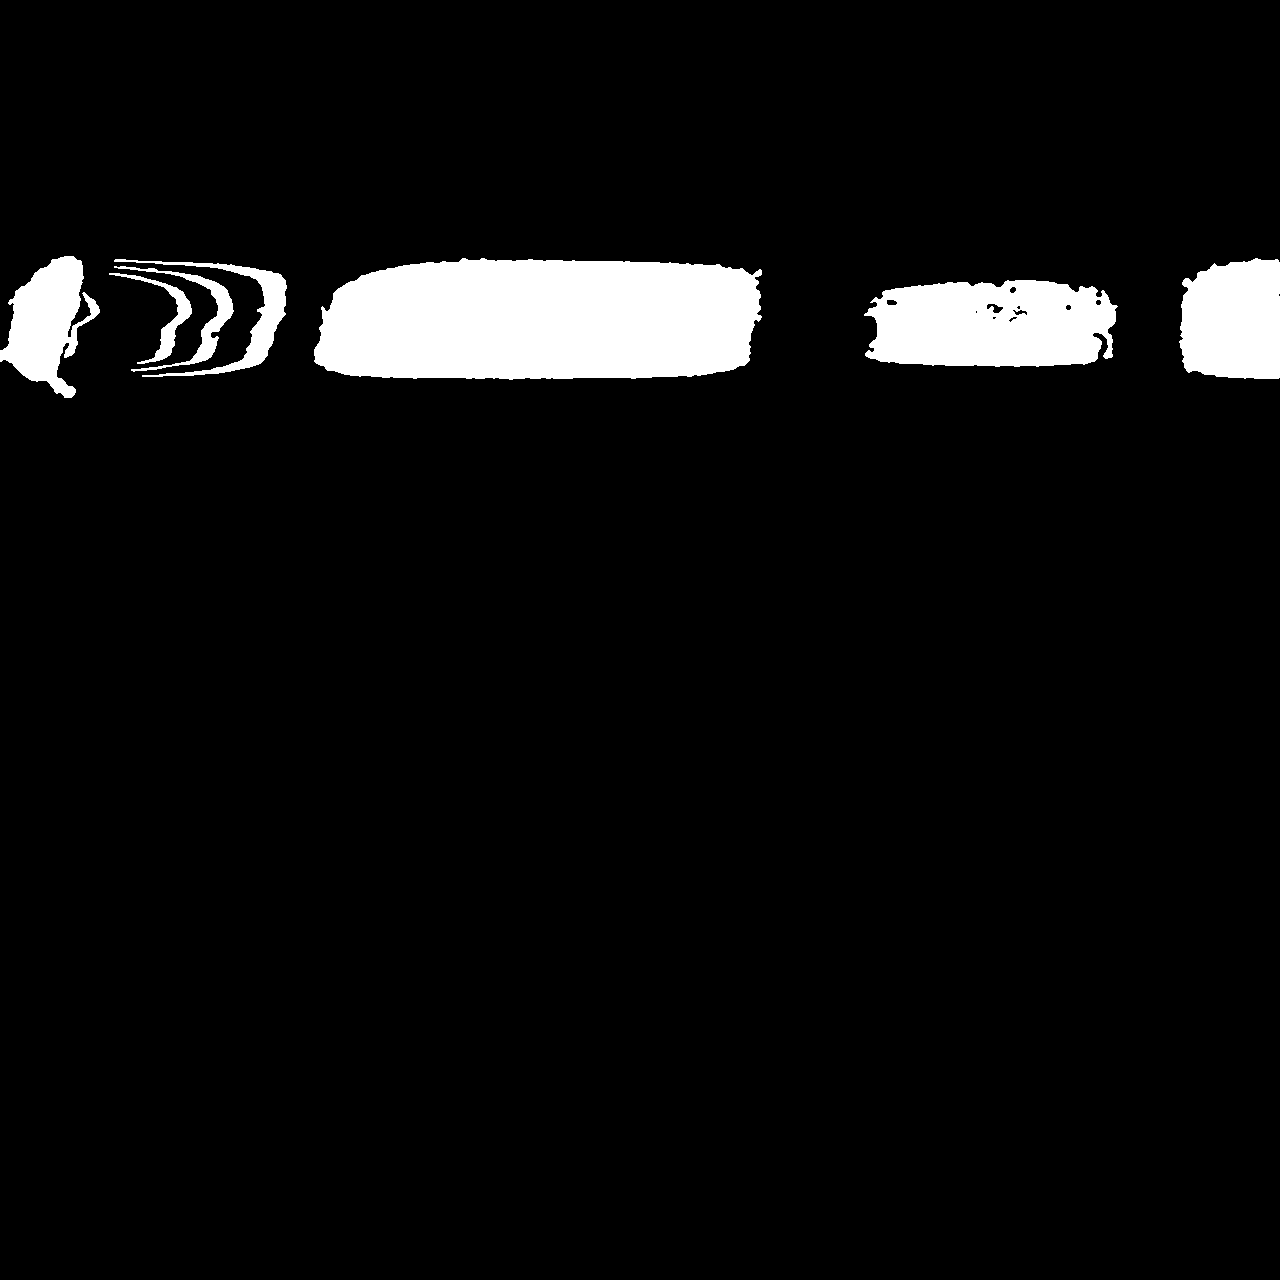
\includegraphics[width=\linewidth]{Maske.png}
		\caption{}
		\label{fig:mask}
	\end{subfigure}%
	\hspace{\fill}
	\begin{subfigure}{0.5\textwidth}
		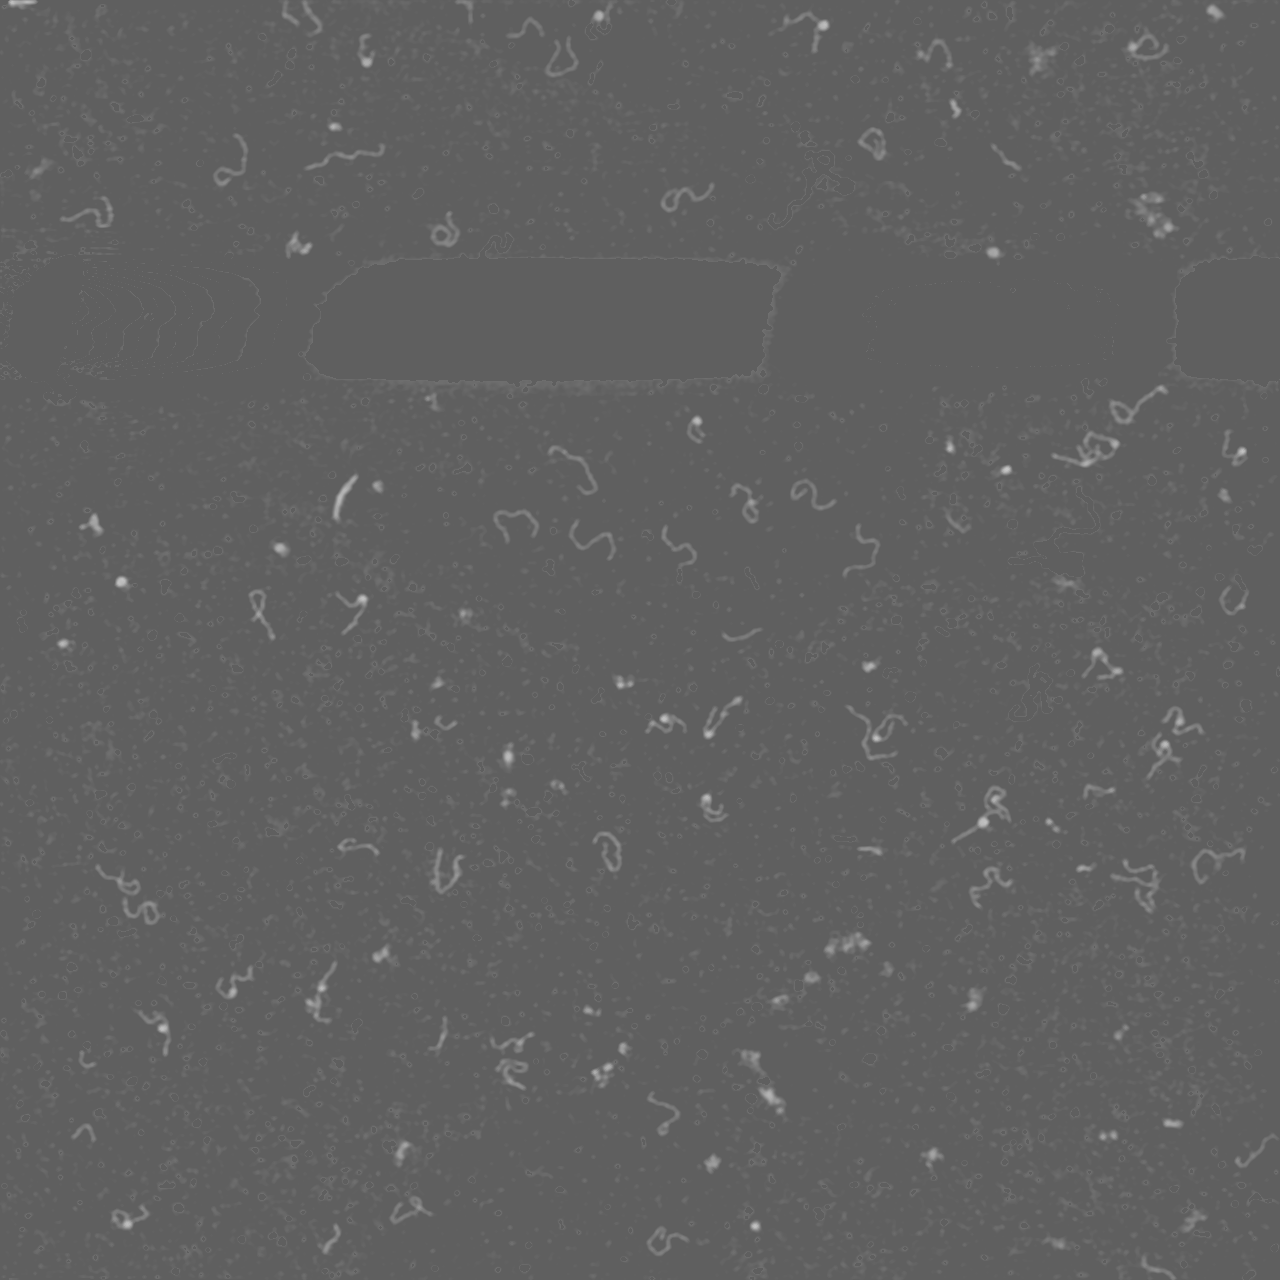
\includegraphics[width=\linewidth]{filtered.png}
		\caption{}
		\label{fig:filtered}
	\end{subfigure}%
	
	\caption{(a)Mask from binary image (b)Mask applied to original image}\label{fig:Process}
\end{figure}
This image is then used as a mask (compare Figure \ref{fig:mask}) which removes all non-DNA objects on the original image from step one.

This means subtract the detected regions on the mask from the original image and set them to the previous determined background level.
The result Figure \ref{fig:filtered} shows how the large outliers are removed and will therefore no longer contribute to the threshold in a negative way.
After this process a second threshold algorithm, in this case the moments threshold (see \ref{sec:Thresholding}), is applied to the original image. 
Duo to the previous steps the new calculated threshold is no longer influenced by background noise or polluted image regions.

In this case the new threshold is now at a intensity value of 111, compared to a intensity value of 135. Figure \ref{fig:compareThresh} shows the improvement in terms of recognized DNA objects on the sample image for type one noise as seen in Figure \ref{fig: Noise1}.
By using this approach it is now possible to analyze pictures with the first type of noise while they had to be discarded entirely before.


\begin{figure}[!htbp]
	\begin{subfigure}{0.5\textwidth}
		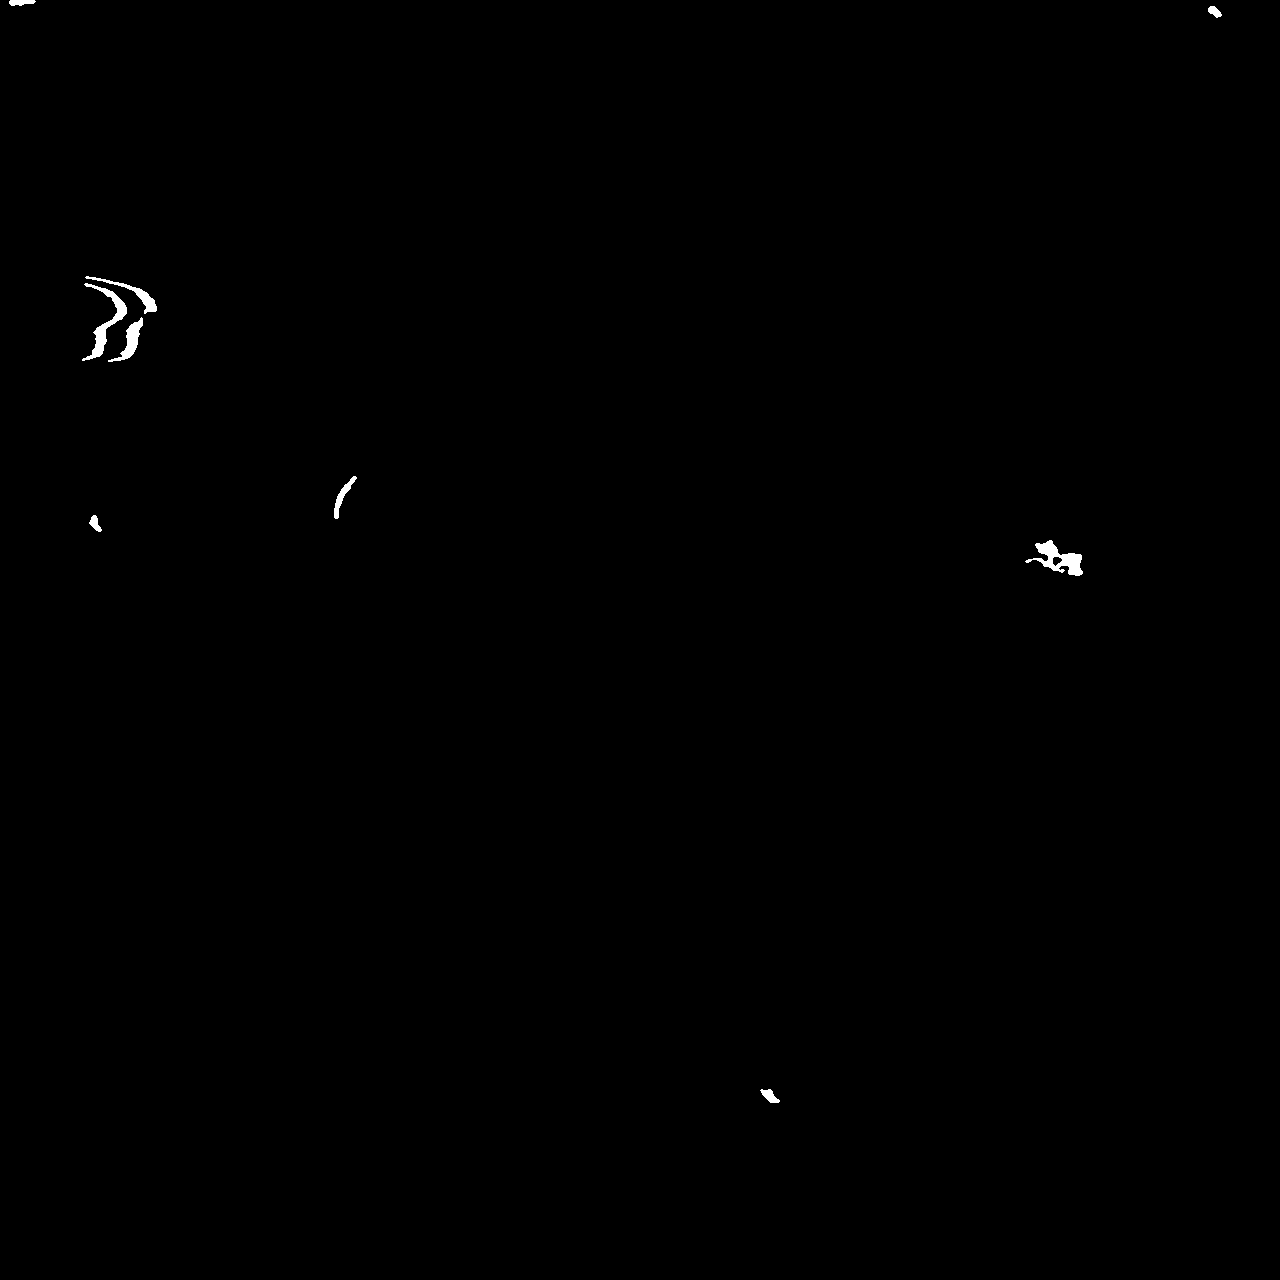
\includegraphics[width=\linewidth]{before.png}
		\caption{Before}
		\label{fig:bwbefore}
	\end{subfigure}%
	\hspace{\fill}
	\begin{subfigure}{0.5\textwidth}
		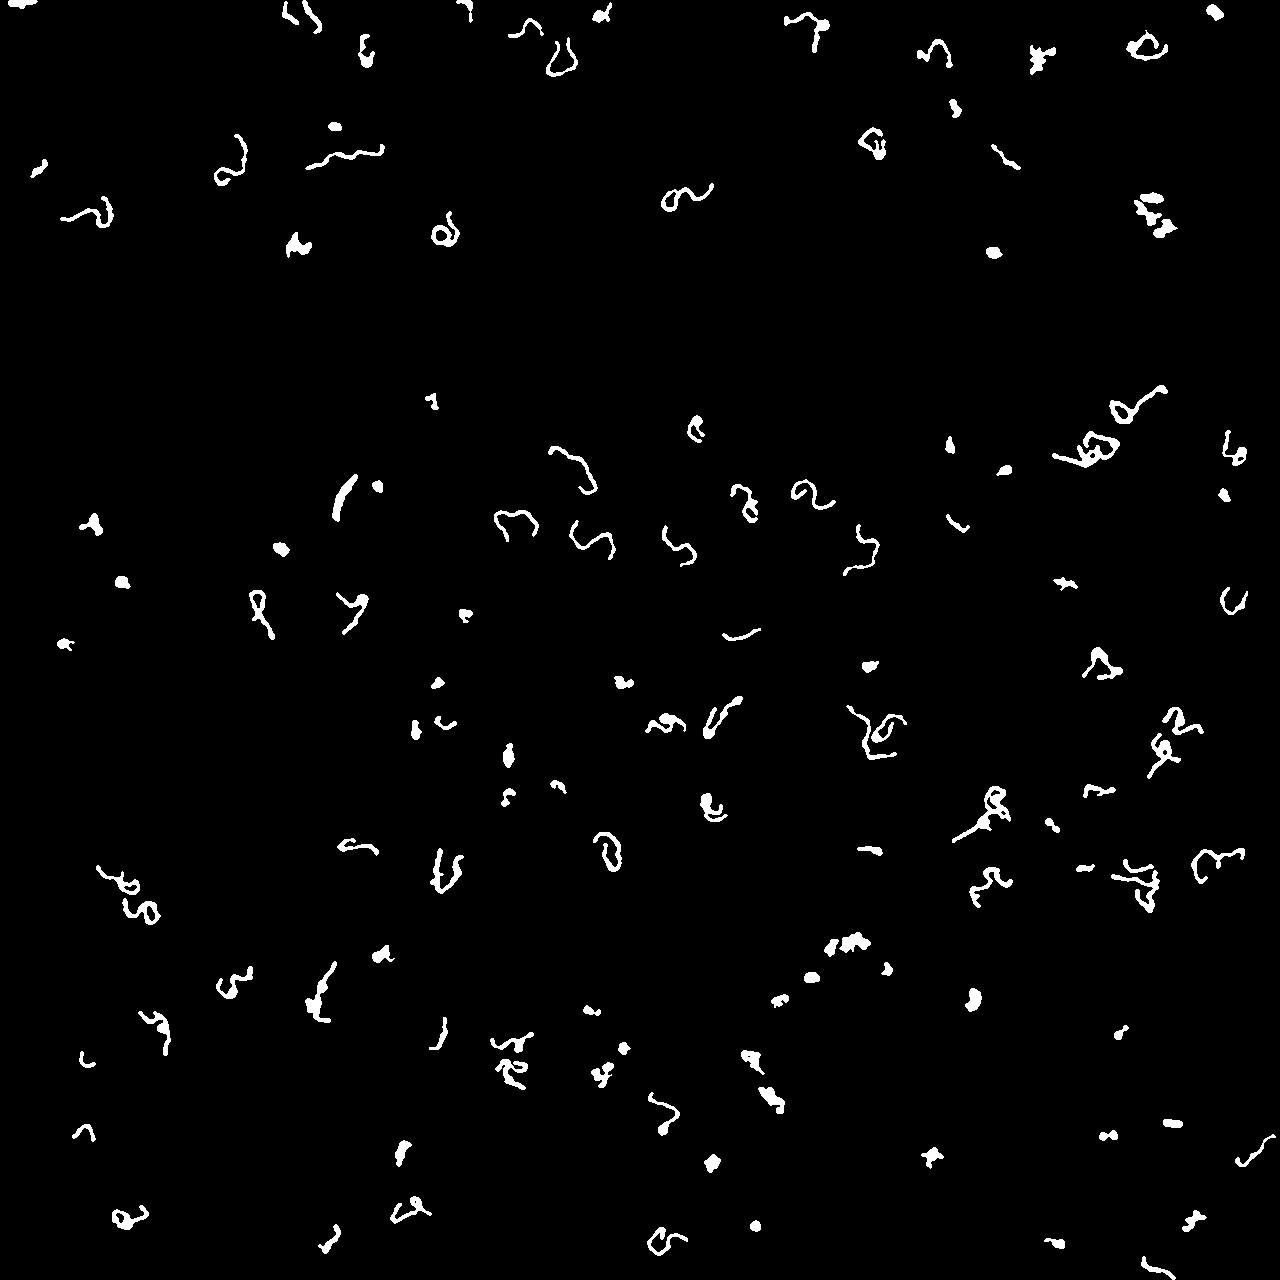
\includegraphics[width=\linewidth]{after.png}
		\caption{After}
		\label{fig:bwafter}
	\end{subfigure}%
	\caption{Comparison with previous method, noise type 1}\label{fig:compareThresh}
\end{figure}

\subsubsection{Limit Threshold}\label{sec: Limit Threshold}
The first two steps focused on keeping the noise and distribution of the height values in a tolerable range on image to image basis. The third and final step of this method aims at limiting the thresholds over the entire dataset.
For this technique a larger dataset of at least 50 images is required.
The histogram of all 105 test images shown in Figure \ref{fig:HistogramThresholds} shows that step one and two already improve the thresholds to a smaller range.
Also, only thresholds, which were too high, have been limited by these steps since only outliers in the upper value range have been treated, while lower values have been set to a fixed background.
The newly calculated thresholds are in a range between 0.4 and 0.46 which corresponds to pixel values of 102 and 117.
Looking at the images with the highest and lowest thresholds, it turns out that they are still prioritizing lower respectively higher pixel values. This results in too small DNA-strands or false positive detections.
In order to limit the probability of these cases the permissible range for thresholds is reduced even further. This is achieved by only allowing thresholds in the range of 1.5 times the standard deviation around the mean of the distribution.
The range is thereby limited to: 
\[
[\bar X - 1.5 * \sigma, \bar X + 1.5 * \sigma] 
\]
\[
= [0.4345-1.5*0.0129, 0.4345+1.5*0.0129] 
= [0.4152,0.4538]\,  % Formel allgemein hinzufügen
\]
All values outside of this interval are set to the nearest boundary.



\begin{figure}[!htb]
	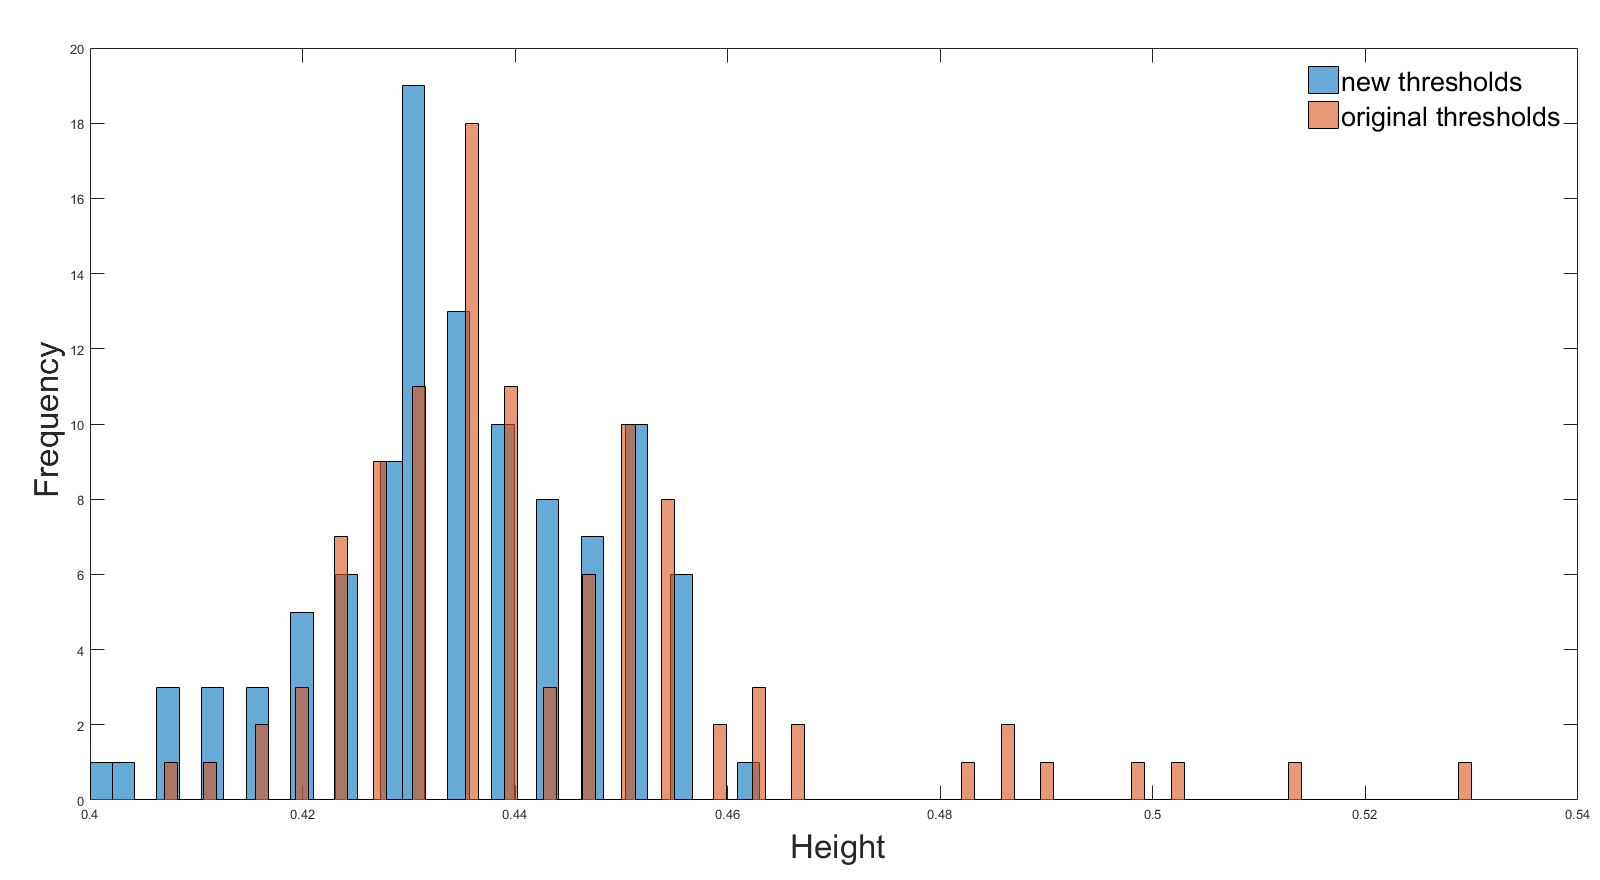
\includegraphics[width=1\linewidth]{thresholds.png}
	\caption{Threshold Distribution over the entire dataset (orange)before and (blue)after step one and two were applied}%formulierung ändern
	\label{fig:HistogramThresholds}
	\end{figure}
	As seen in Figure \ref{fig:compareThresh} this method effectively detects and removes polluted image regions and ensures a high DNA-strand detection on images with noise type one.
Due to the nature and height field of noise of type two this approach can only limit false detections to a certain degree (see Figure \ref{fig:compareThresh1}).
Although it was not expected to work on this kind of imperfections at all. While almost all DNA-strands are detected correctly some false positive still exist.
In conclusion, the proposed approach improves image quality and detection rate on very noisy images greatly while leaving already well processed images the way they are.

\begin{figure}[!htbp]
	\begin{subfigure}{0.5\textwidth}
		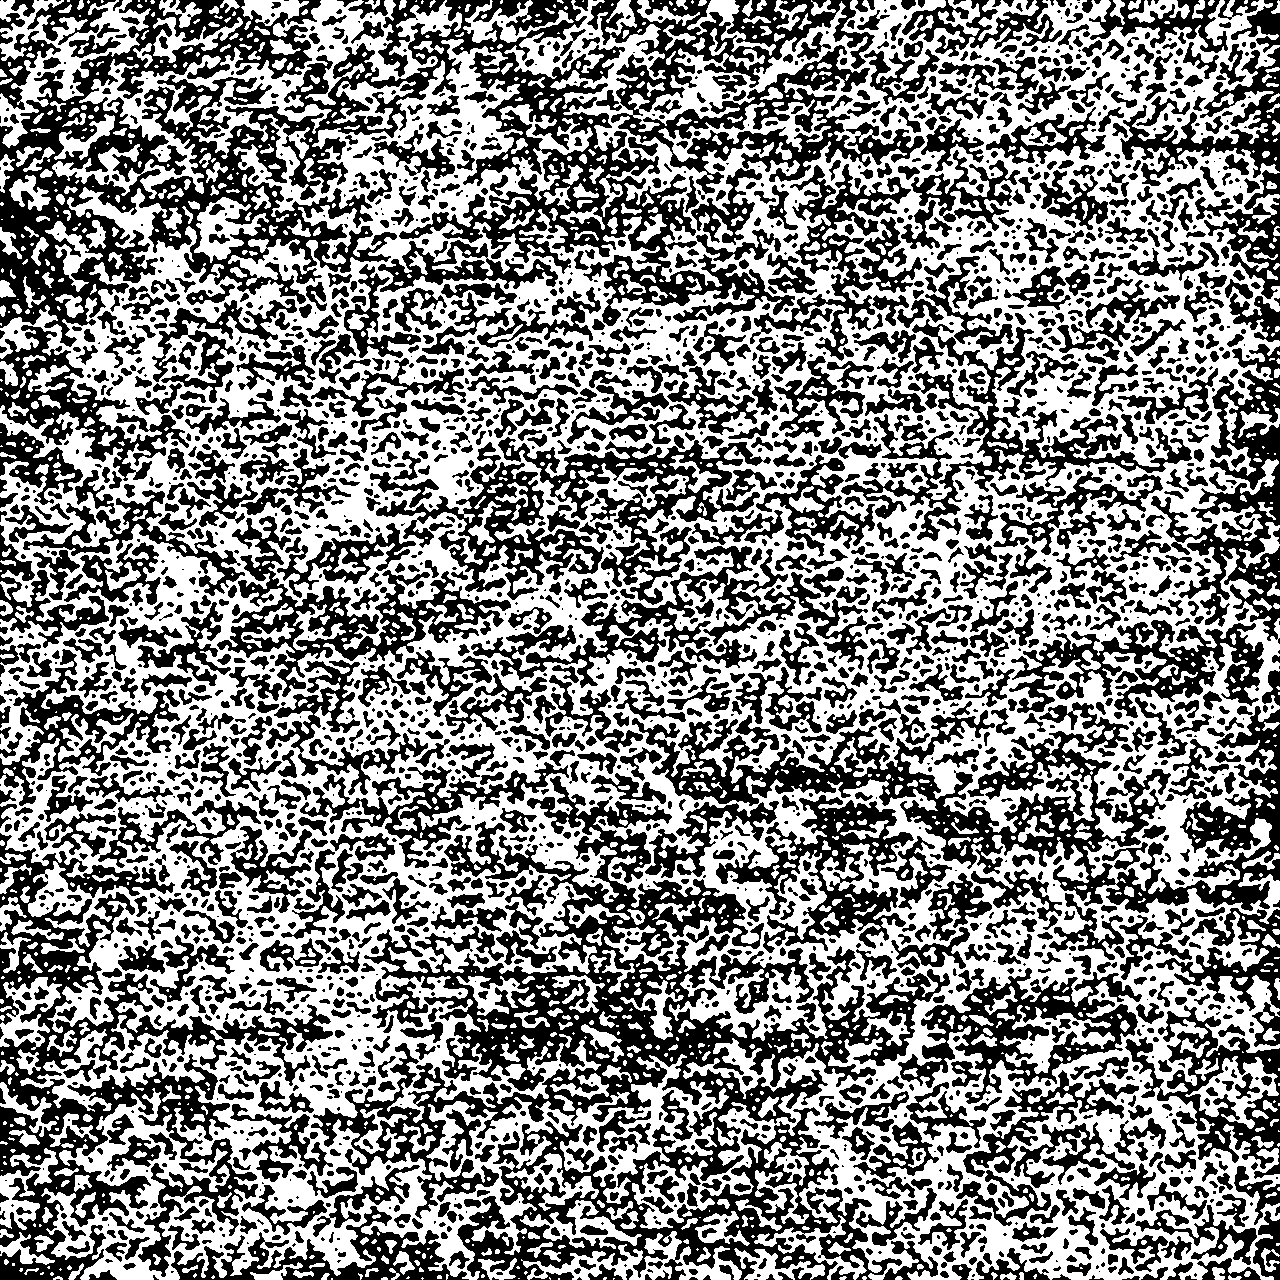
\includegraphics[width=\linewidth]{noise2before.png}
		\caption{Before}
		\label{fig:bwbefore}
	\end{subfigure}%
	\hspace{\fill}
	\begin{subfigure}{0.5\textwidth}
		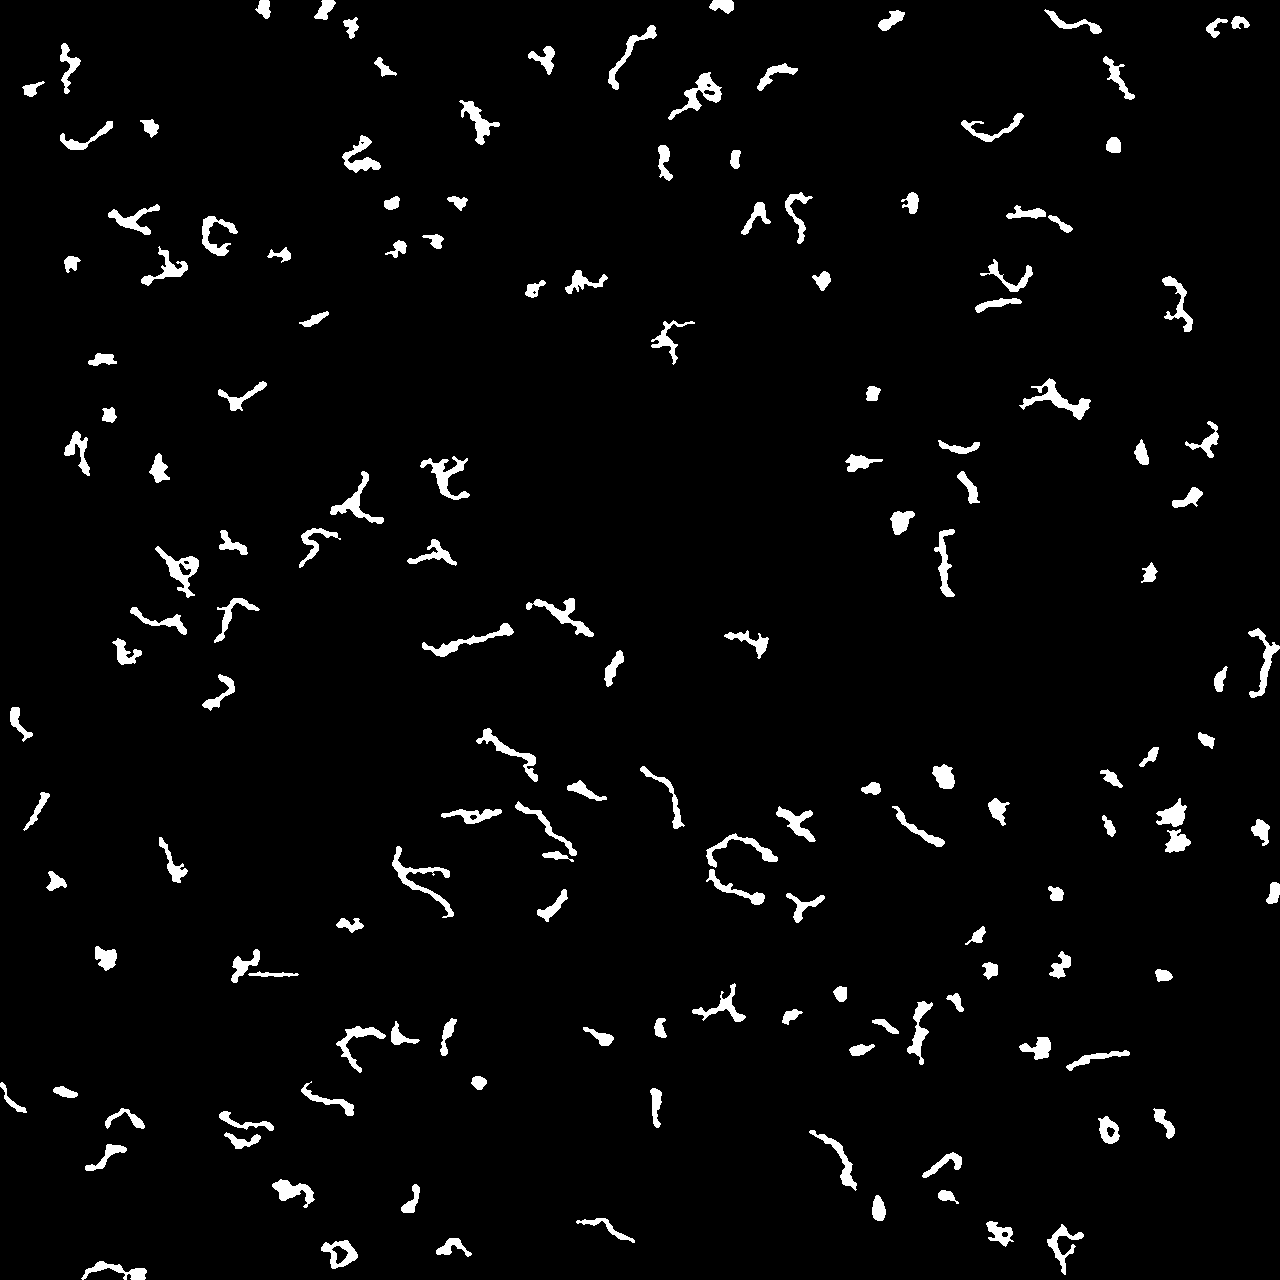
\includegraphics[width=\linewidth]{noise2after.png}
		\caption{After}
		\label{fig:bwafter}
	\end{subfigure}%
	\caption{Comparison with previous method, noise type 2}\label{fig:compareThresh1}
\end{figure}
\newpage
